\documentclass[dvipdfmx]{jarticle}
\pagestyle{empty}
\usepackage{tikz}
\usetikzlibrary{shapes,arrows.meta,calc}
\begin{document}
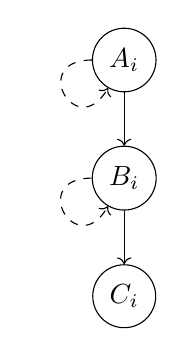
\begin{tikzpicture}
\node[draw,circle] (N1) at (0,0) {$A_i$};
\node[draw,circle] (N2) at (0,-1.5) {$B_i$};
\node[draw,circle] (N3) at (0,-3) {$C_i$};
\path[->] (N1) edge (N2) (N2) edge (N3);
\path[->] (N1) [loop left,out=180,in=240,looseness=5,style=dashed] edge (N1);
\path[->] (N2) [loop left,out=180,in=240,looseness=5,style=dashed] edge (N2);
\end{tikzpicture}
\end{document}